\section{Algorithm}

\sectionPage{Algorithm}

\begin{frame}[c]{Algorithm}{}
    \begin{enumerate}
        \setcounter{enumi}{1}
        \item Algorithm
            \begin{enumerate}
                \item Filter
                \item RMS
            		\begin{enumerate}
                		\item Time Coefficients     
            		\end{enumerate}
                \item Gate
                \item Gain
            		\begin{enumerate}
					\item Loudness Goal Adaption  
					\item Write Automation  
            		\end{enumerate}
                \item Lookahead
            \end{enumerate}
    \end{enumerate}
\end{frame}

\begin{frame}[c]{Algorithm: Filter}{}
	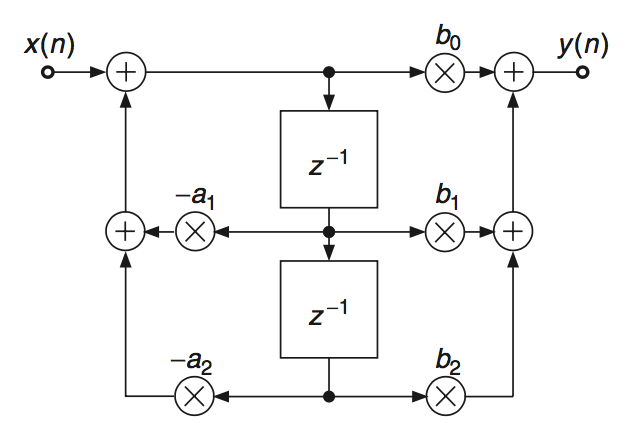
\includegraphics[scale=0.3]{images/biquat}
	\centering
    \footfullcite{Figure from DAFX: Digital Audio Effects by Udo Zoelzer}

    \printbibliography%
\end{frame}

\begin{frame}[c]{Algorithm: Filter}{}
	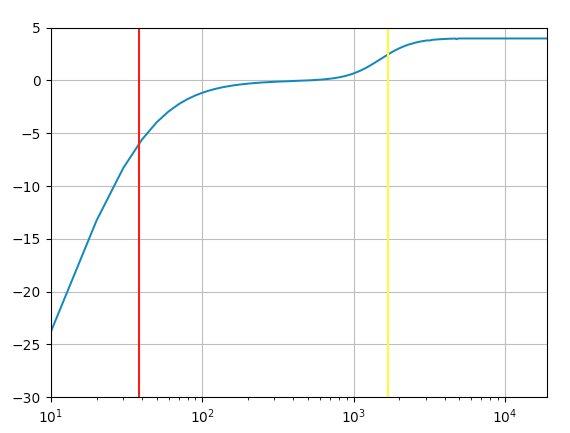
\includegraphics[scale=0.3]{images/filter}
	\centering\\
	\bigskip
    \begin{itemize}
    		\item lowcut (38 Hz), highshelf (1681 Hz) \footfullcite{from Recommendation ITU-R BS.1770-4}
    \end{itemize}

    \printbibliography%
\end{frame}

\begin{frame}[fragile]{Algorithm: RMS}{}
	Root Mean Square (RMS):
	\lstset{language=C++}
	\begin{lstlisting}[basicstyle=\tiny]
void AutoVocalCtrlAudioProcessor::updateRMS(int channel)
{
    rms[channel] = (1. - rmsCo) * rms[channel] +
                   rmsCo * (filterSample[channel] * filterSample[channel]);
}
	\end{lstlisting}
	\footfullcite{Based on Book: Digital Audio Signal Processing by Udo Zoelzer}\\
	\bigskip
	Time Constants:
	\begin{lstlisting}[basicstyle=\tiny]
float AutoVocalCtrlAudioProcessor::getTimeConstant(float ms)
{
    if (ms > 0.f)
        return 1.f - exp(-2.2*(1./currentSampleRate)/(ms/1000.));
    else
        return 1.f;
}
	\end{lstlisting}
	\footnotemark[2]
	
    \printbibliography%
\end{frame}

\begin{frame}[c]{Algorithm: Gate}{}
	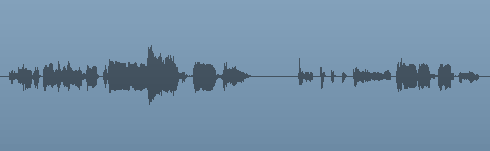
\includegraphics[scale=0.6]{images/wave}
	\centering
\end{frame}

\begin{frame}[fragile]{Algorithm: Gain}{}
	\lstset{language=C++}
	\begin{lstlisting}[basicstyle=\tiny]
void AutoVocalCtrlAudioProcessor::updateGain(int channel)
{
    const double g = *loudnessGoal - mls[channel];
    const double co = g < gain[channel] ? compressTCo:expandTCo;
    gain[channel] = clipRange.clipValue((1 - co) * gain[channel] + co * g);
    updateAutomation();
    ...
}
	\end{lstlisting}
\end{frame}

\begin{frame}[fragile]{Algorithm: Gain: Loudness Goal Adaption}{}
	\lstset{language=C++}
	\begin{lstlisting}[basicstyle=\tiny]
void AutoVocalCtrlAudioProcessor::updateGain(int channel)
{
    ...
    alphaGain[channel] = (1 - alphaCo) * alphaGain[channel] + alphaCo * gain[channel];
    if (channel == getTotalNumInputChannels() - 1)
    {
        ...
        updateLoudnessGoal();
    }
}
	\end{lstlisting}
\end{frame}

\begin{frame}[fragile]{Algorithm: Gain: Write Automation}{}
	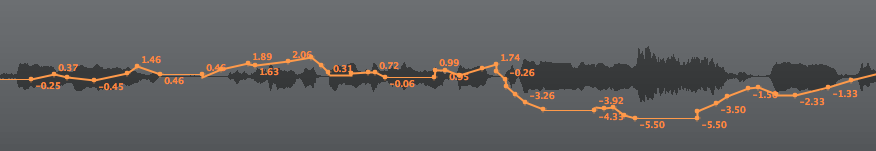
\includegraphics[scale=0.365]{images/automation}
	\centering
\end{frame}

\begin{frame}[c]{Algorithm: Lookahead}{per ringbuffer}
	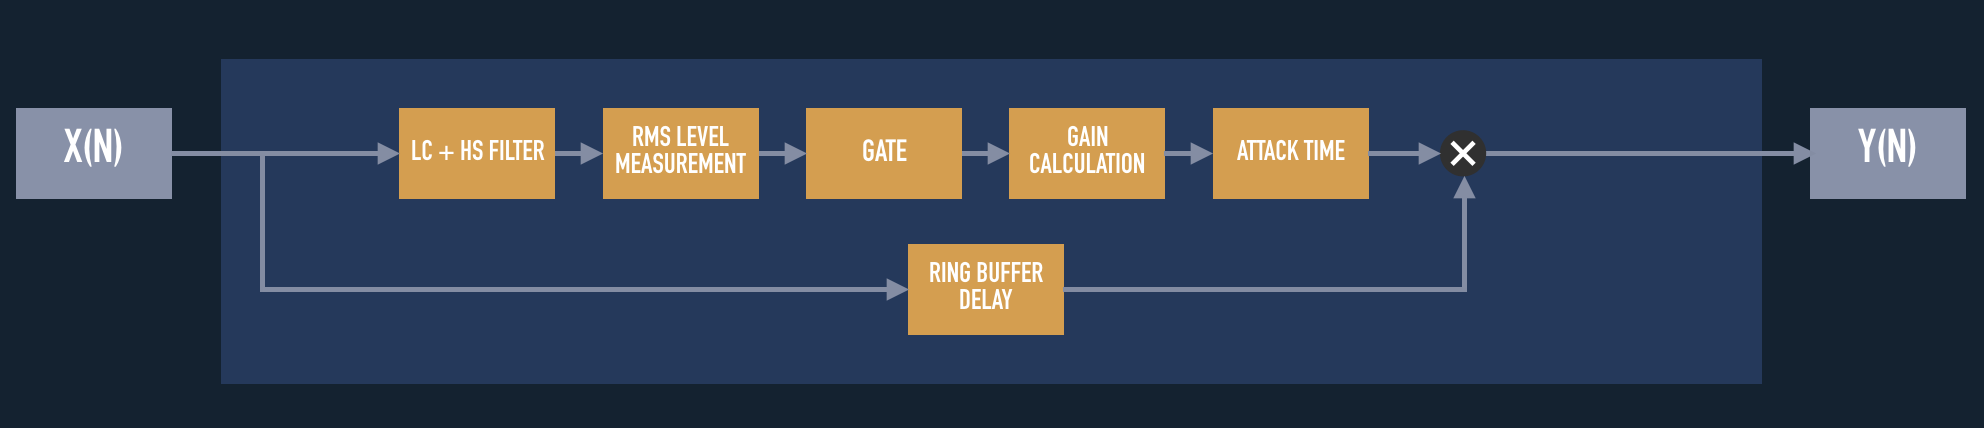
\includegraphics[scale=0.32]{images/lookahead}
	\centering
	\\
\end{frame}